\section*{Question 3}


A thin rod of length $L$ lies along the $x$-axis extending from $x = 0$ to $x = L$. The rod carries a nonuniform linear charge density given by
\begin{equation*}
    \lambda(x) = \lambda_0 \frac{x}{L}
\end{equation*}
where $\lambda_0$ is a constant with units of charge per unit length.
\begin{center}
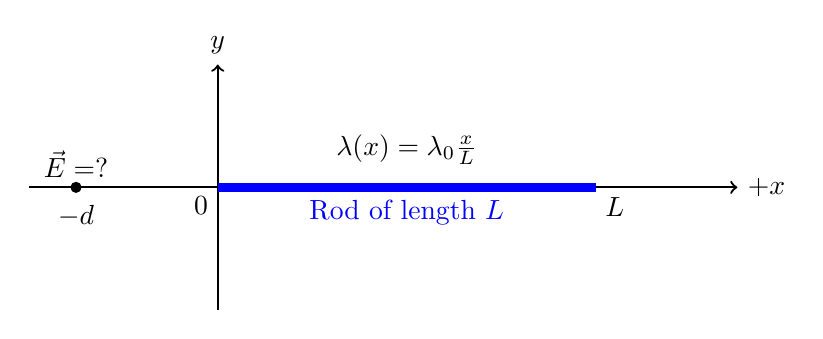
\begin{tikzpicture}[scale=1.2]
    % Draw the x-axis
    \draw[->, thick] (-2,0) -- (5.5,0) node[right] {$+x$};
    
    % Draw the y-axis
    \draw[->, thick] (0,-1.3) -- (0,1.3) node[above] {$y$};
    
    % Draw the thin rod from x=0 to x=L (here L is represented as a finite segment)
    \draw[line width=3pt, blue] (0,0) -- (4,0) node[midway, below] {Rod of length $L$};
    
    % Mark the endpoints of the rod
    \draw[fill] (0,0)  node[below left] {$0$};
    \draw[fill] (4,0)  node[below right] {$L$};
    
    % Add annotation for the nonuniform charge density along the rod
    \node at (2, 0.4) {$\lambda(x)=\lambda_0\frac{x}{L}$};
    
    % Position the test charge Q at x = -d (assuming d>0, here set d=1.5 for clarity)
    \draw[fill] (-1.5,0) circle (1.5pt) node[above] {$\vec{E}=?$};
    
    % Optional: annotate the x-coordinate of the field point
    \node at (-1.5, -0.3) {$-d$};
\end{tikzpicture}
\end{center}

\begin{enumerate}
    \item[(a)] Write down the differential contribution $d\vec{E}$ of an infinitesimal charge element $dq$ located at position $x$ on the rod to the electric field at $x=-d$. --- \textit{0.6 pts}
    \item[(b)] What is the net electric field $\vec{E}$ at $x=-d$ due to the entire rod?. --- \textit{0.4 pts}
\end{enumerate}

\underline{Given:}
\begin{itemize}
    \item $\int_{0}^{x_0} \frac{x dx}{(a+x)^2} = \left[ \ln\left(\frac{a+x_0}{a}\right) + \frac{a}{a+x_0} -1 \right]$, where $x_0>0$ and $a>0$ are constants.
\end{itemize}



\section*{Solution:}

